
% płeć
\begin{figure}
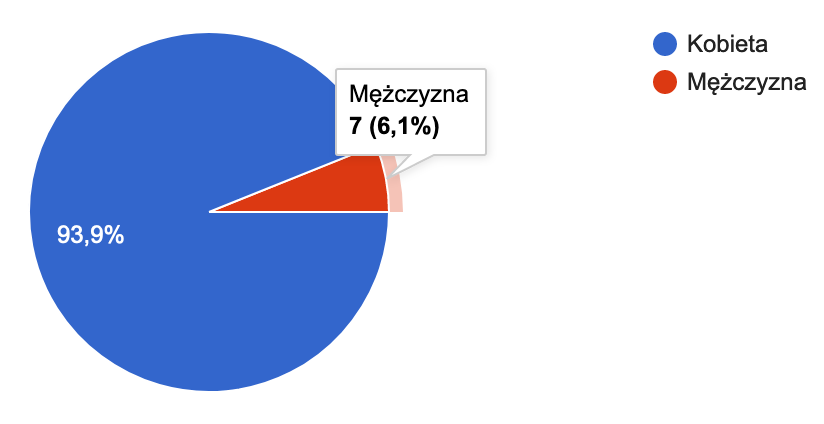
\includegraphics[width=8cm]{char_gr_bad/plec00}
\caption{Płeć}
\end{figure}

% wiek
\begin{figure}
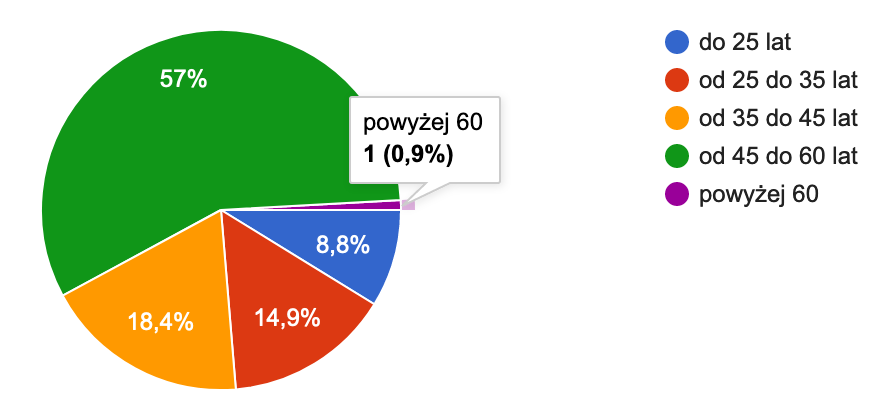
\includegraphics[width=8cm]{char_gr_bad/wiek00}
\caption{Wiek}
\end{figure}

% wykształcenie
\begin{figure}
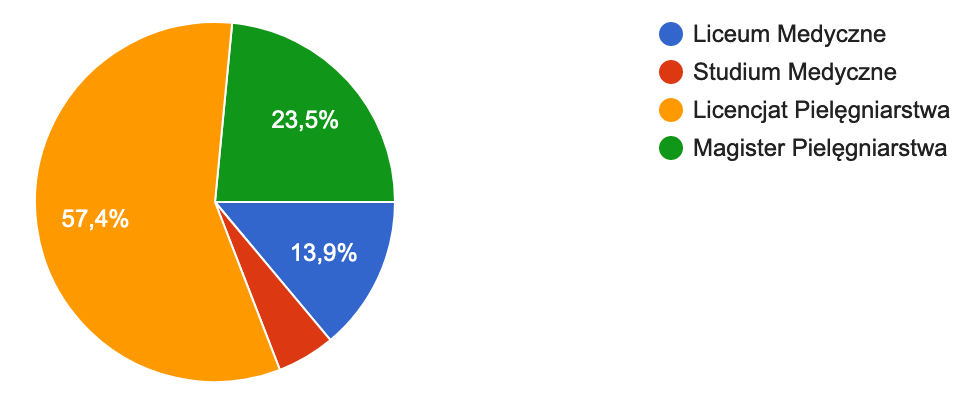
\includegraphics[width=9cm]{char_gr_bad/wyksztalc00}
\caption{Wykształcenie}
\end{figure}

% podyplomowe
\begin{figure}
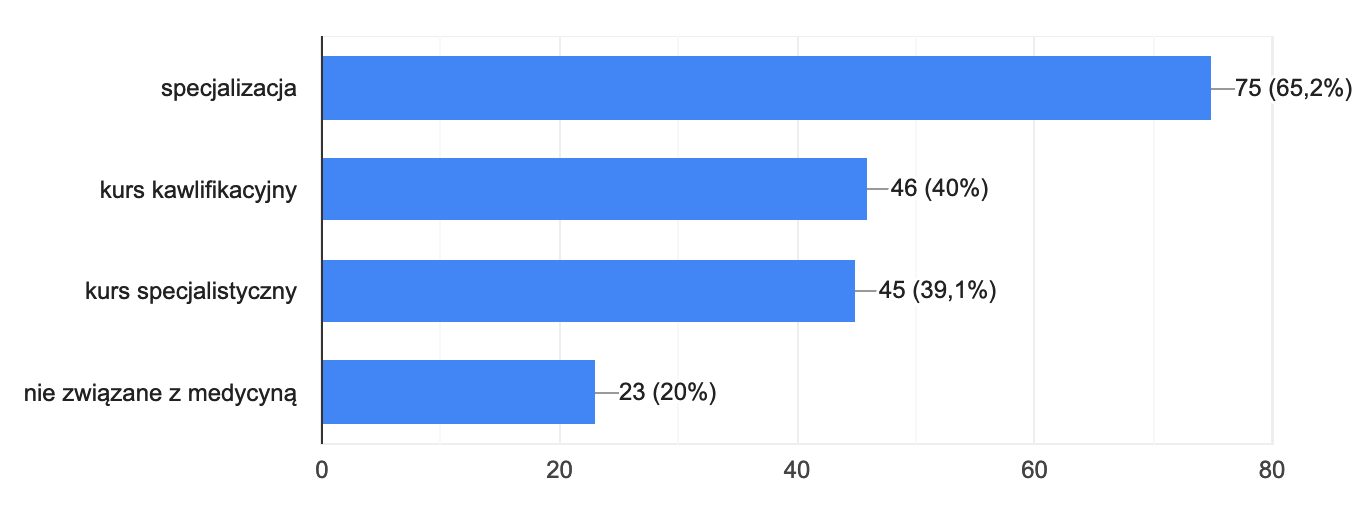
\includegraphics[width=10cm]{char_gr_bad/podyplom00}
\caption{Kształcenie podyplomowe}
\end{figure}

% stan cywilny
\begin{figure}
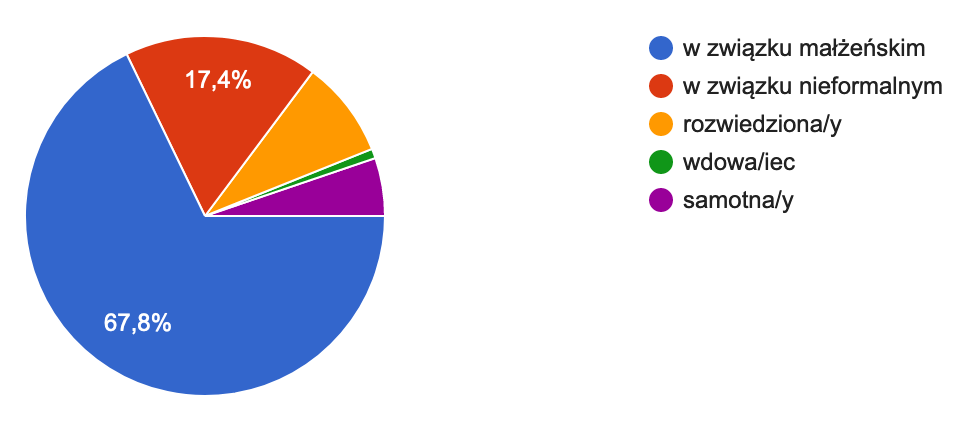
\includegraphics[width=9cm]{char_gr_bad/cyw00}
\caption{Stan cywilny}
\end{figure}

% miejsce zamieszkania
\begin{figure}
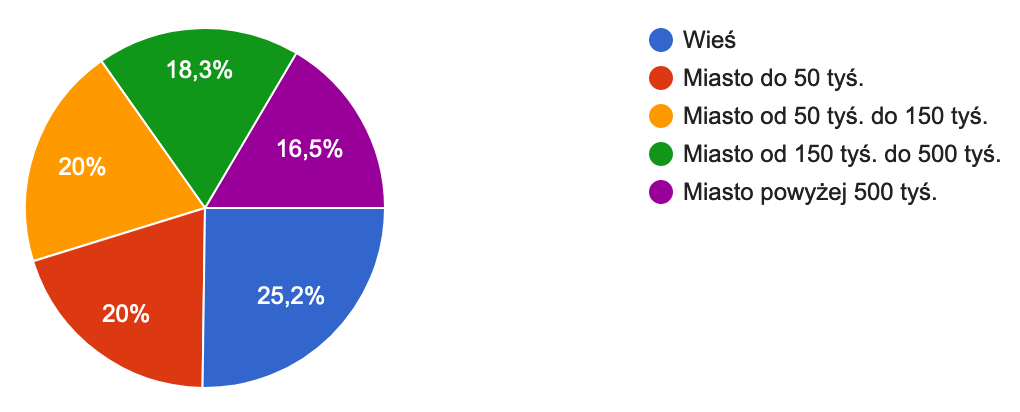
\includegraphics[width=9cm]{char_gr_bad/zamieszka00}
\caption{Miejsce zamieszkania}
\end{figure}


\newpage


\section{Wyniki ankiety}

%  01 staz pracy
\begin{figure}
    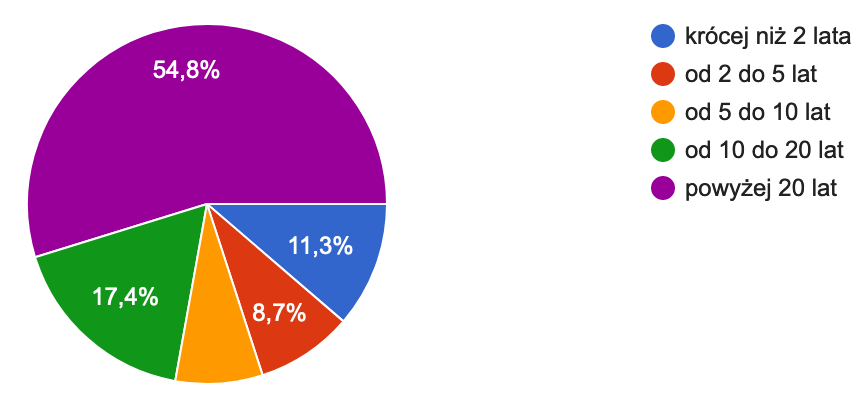
\includegraphics[width=9cm]{wyniki/01_staz_pracy}
    \caption{Jak długo pracuje Pan/i w zawodzie pielęgniarki/rza?}
    \label{rys:staz}
\end{figure}

%  02 ile miejsc
\begin{figure}
    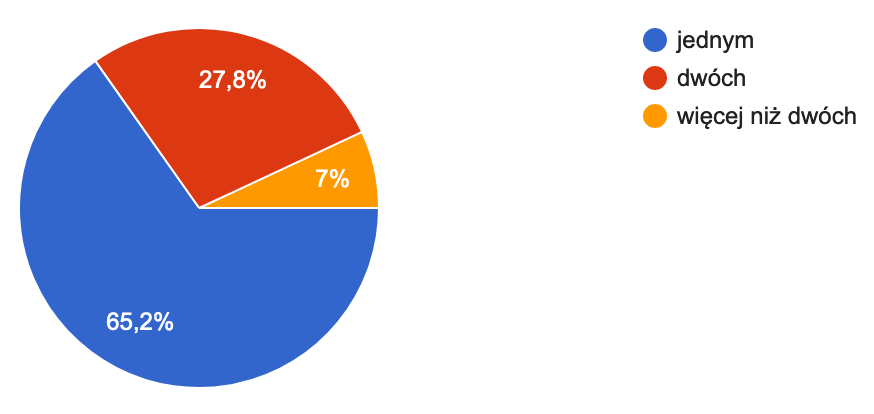
\includegraphics[width=9cm]{wyniki/02_ile_miejsc}
    \caption{W ilu miejscach pracy, obecnie Pan/i jest zatrudniony/a?}
    \label{rys:etaty}
\end{figure}

%  03 wymiar godzin
\begin{figure}
    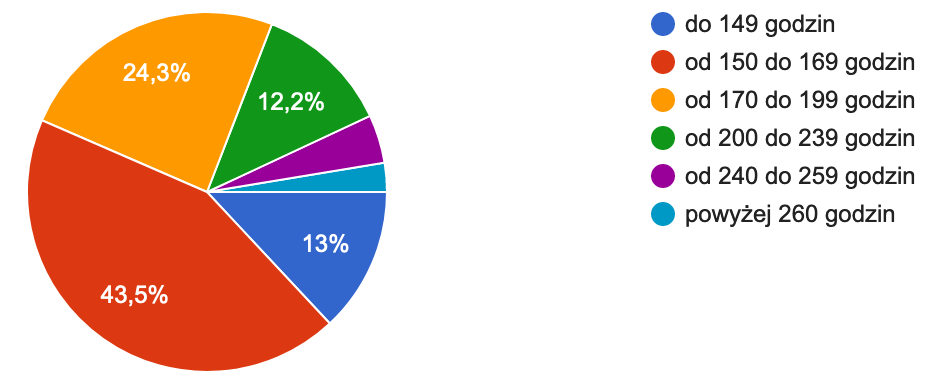
\includegraphics[width=9cm]{wyniki/03_wymiar_godzin}
    \caption{Ile wynosi miesięczny wymiar godzin, Pana/i pracy?}
    \label{rys:ile_godzin}
\end{figure}

%  04 ile zmian
\begin{figure}
    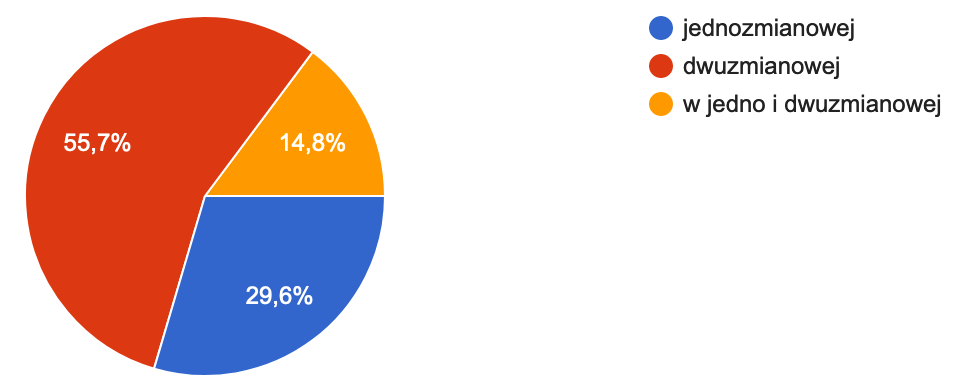
\includegraphics[width=9cm]{wyniki/04_ile_zmian}
    \caption{Czy w podstawowym miejscu zatrudnienia, świadczy  Pan/i usługi, w systemie pracy?}
    \label{rys:ile_zmian}
\end{figure}

%  05 zadowol
\begin{figure}
    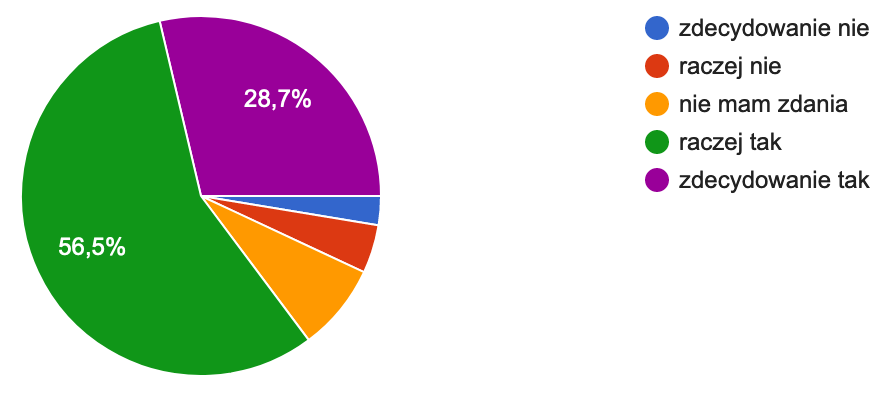
\includegraphics[width=9cm]{wyniki/05_zadowol}
    \caption{Czy jest Pan/i zadowolony/a, z wyboru drogi zawodowej?}
    \label{rys:zadowol}
\end{figure}

%  06 staz w spec
\begin{figure}
    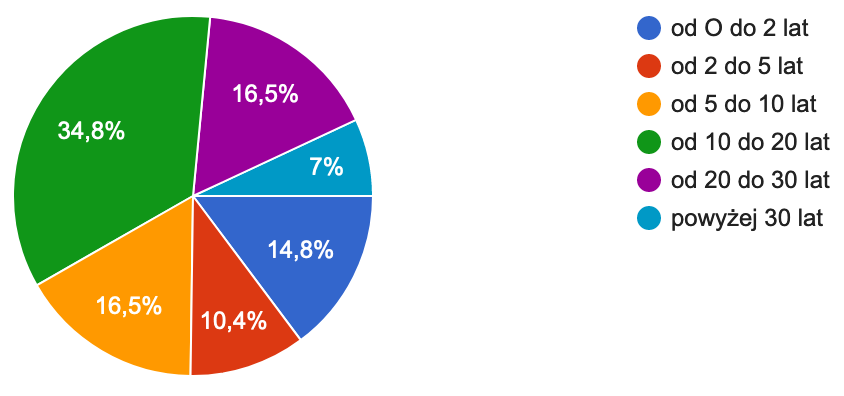
\includegraphics[width=9cm]{wyniki/06_staz_w_spec}
    \caption{Proszę podać, w przybliżeniu staż pracy, w jednej specjalizacji zawodowej (na jednym oddziale)}
    \label{rys:staz_spec}
\end{figure}

%  07 srod wspiera
\begin{figure}
    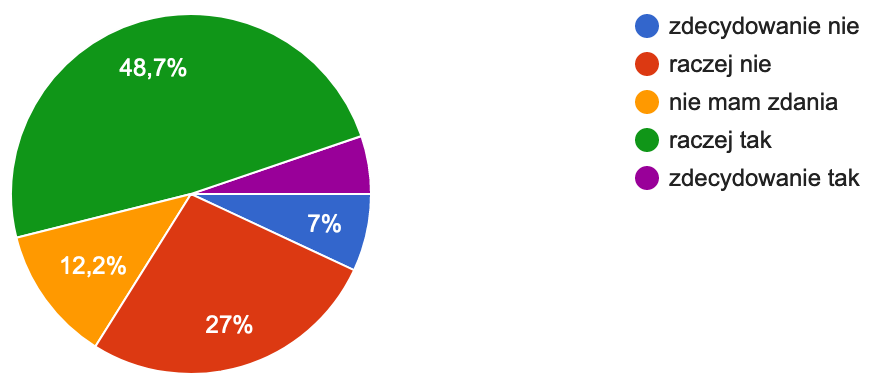
\includegraphics[width=9cm]{wyniki/07_srod_wspiera}
    \caption{Czy środowisko Pana/i pracy, jest wspierające?}
    \label{rys:wspiera}
\end{figure}

%  08 srod toksyczne
\begin{figure}
    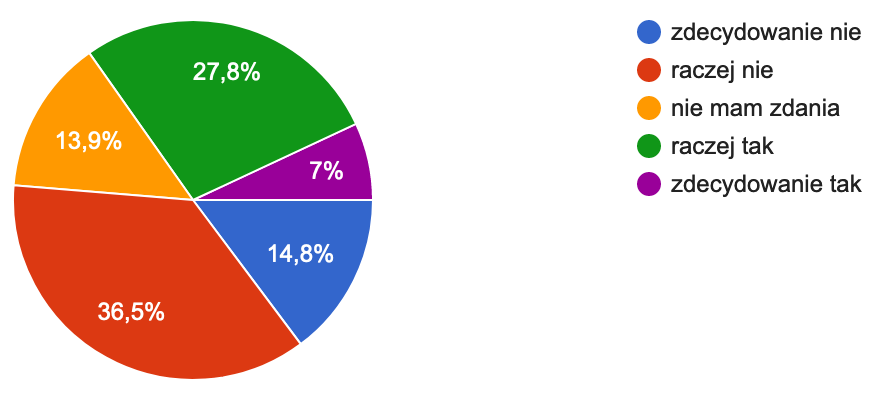
\includegraphics[width=9cm]{wyniki/08_srod_toksyczne}
    \caption{Czy środowisko Pana/i pracy, jest ,,toksyczne"( występuje mobbing,hejt)?}
    \label{rys:toksyczne}
\end{figure}

%  09 systemy motyw
\begin{figure}
    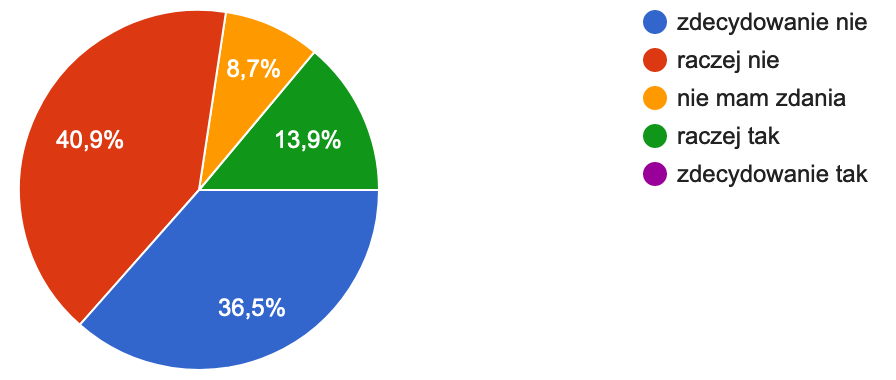
\includegraphics[width=9cm]{wyniki/09_systemy_motyw}
    \caption{Czy zakład pracy, w którym Pan/i pracuje, stosuje systemy motywacyjne?}
    \label{rys:syst_motyw}
\end{figure}

%  10 emocje do domu
\begin{figure}
    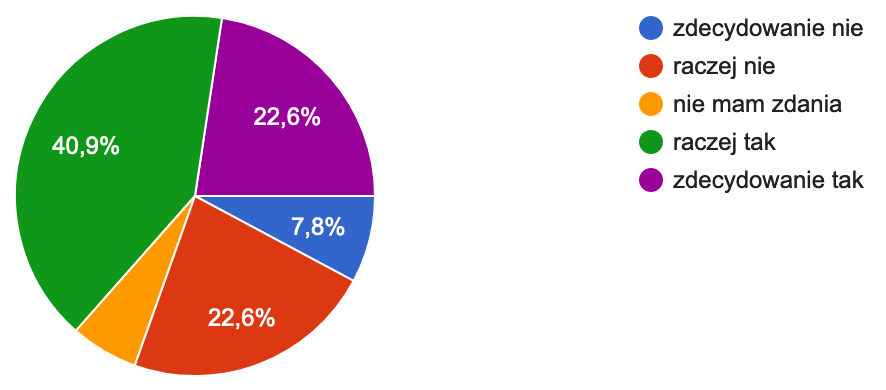
\includegraphics[width=9cm]{wyniki/10_emocje_do_domu}
    \caption{ 10 emocje do domu }
\end{figure}

%  11 trauma wtorna
\begin{figure}
    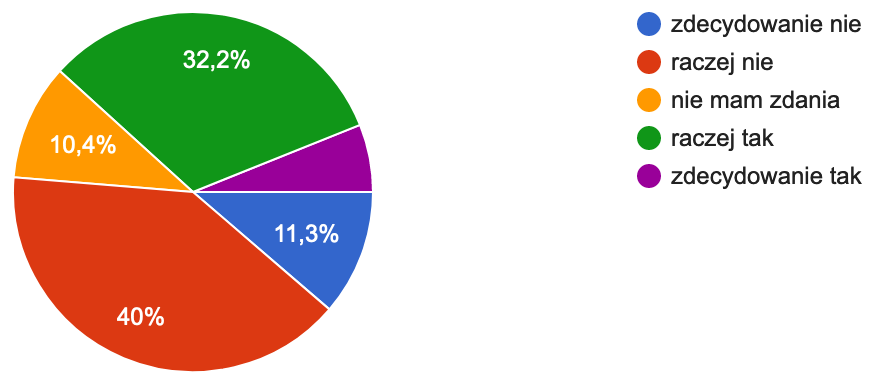
\includegraphics[width=9cm]{wyniki/11_trauma_wtorna}
    \caption{ 11 trauma wtorna }
\end{figure}

%  12 potrafi niwelowac
\begin{figure}
    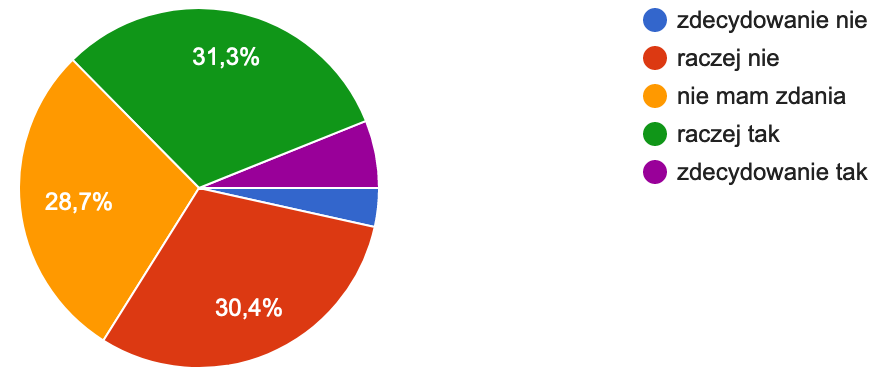
\includegraphics[width=9cm]{wyniki/12_potrafi_niwelowac}
    \caption{ 12 potrafi niwelowac }
\end{figure}

%  13 siega po uzywki
\begin{figure}
    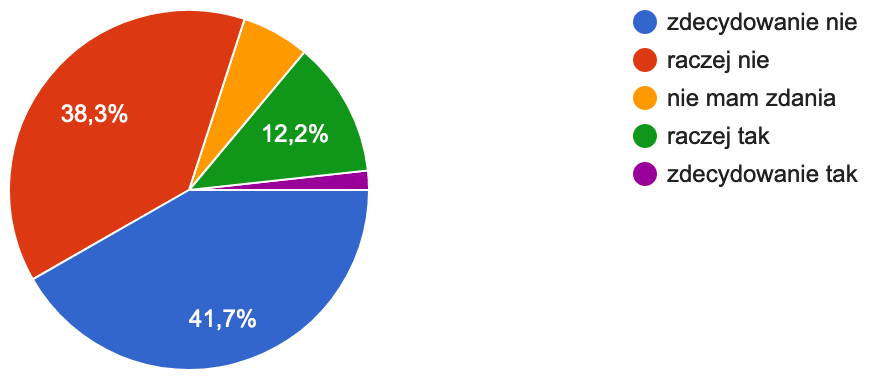
\includegraphics[width=9cm]{wyniki/13_siega_po_uzywki}
    \caption{ 13 siega po uzywki }
\end{figure}

%  14 dylemat podnos kwal
\begin{figure}
    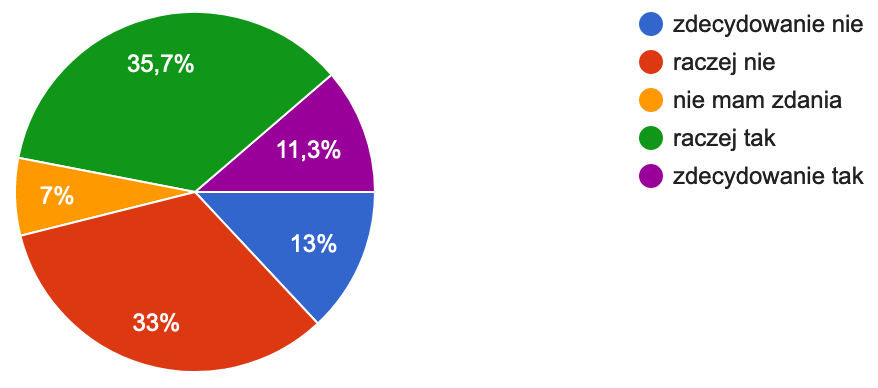
\includegraphics[width=9cm]{wyniki/14_dylemat_podnos_kwal}
    \caption{ 14 dylemat podnos kwal }
\end{figure}

%  15 presja spol
\begin{figure}
    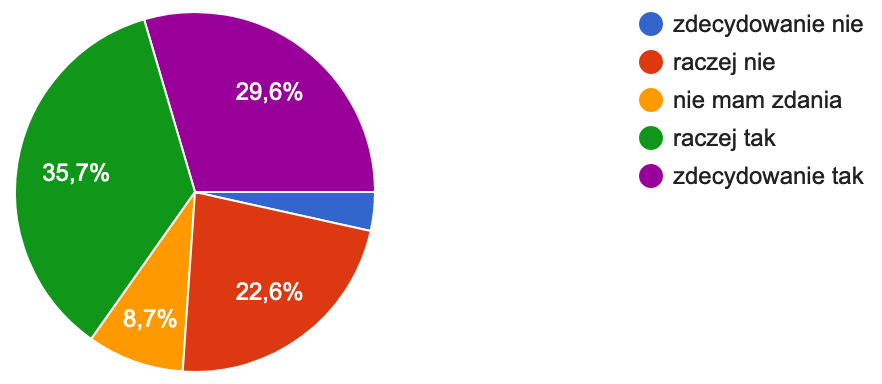
\includegraphics[width=9cm]{wyniki/15_presja_spol}
    \caption{ 15 presja spol }
\end{figure}

%  16 dosw przemoc
\begin{figure}
    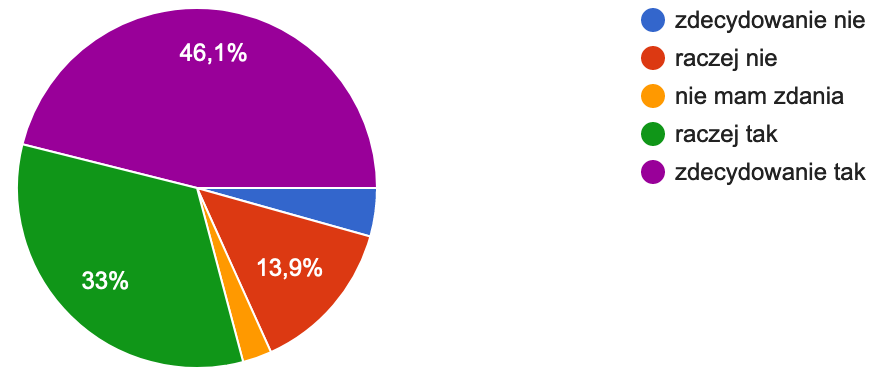
\includegraphics[width=9cm]{wyniki/16_dosw_przemoc}
    \caption{ 16 dosw przemoc }
\end{figure}

%  17 postep dochodz
\begin{figure}
    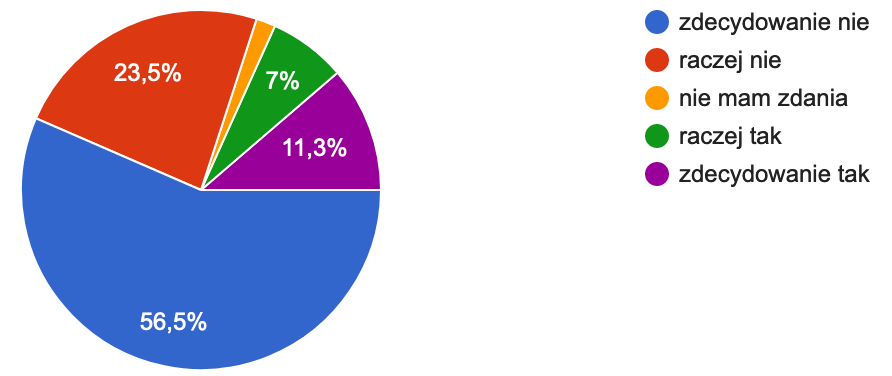
\includegraphics[width=9cm]{wyniki/17_postep_dochodz}
    \caption{ 17 postep dochodz }
\end{figure}

%  18 pocz bezp covid
\begin{figure}
    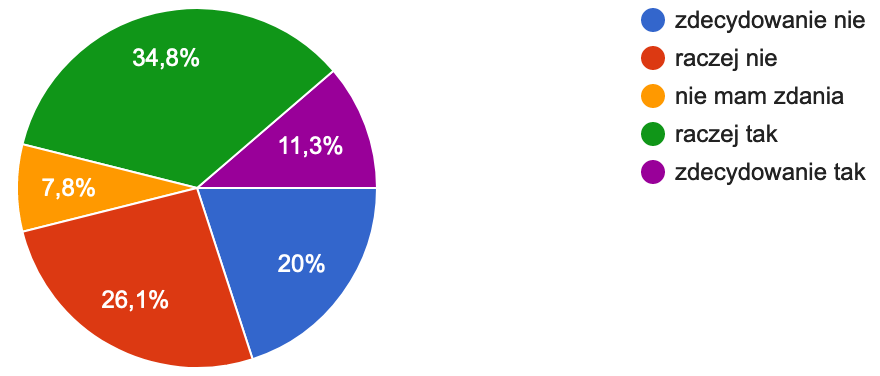
\includegraphics[width=9cm]{wyniki/18_pocz_bezp_covid}
    \caption{ 18 pocz bezp covid }
\end{figure}

%  19 popiera dzialania
\begin{figure}
    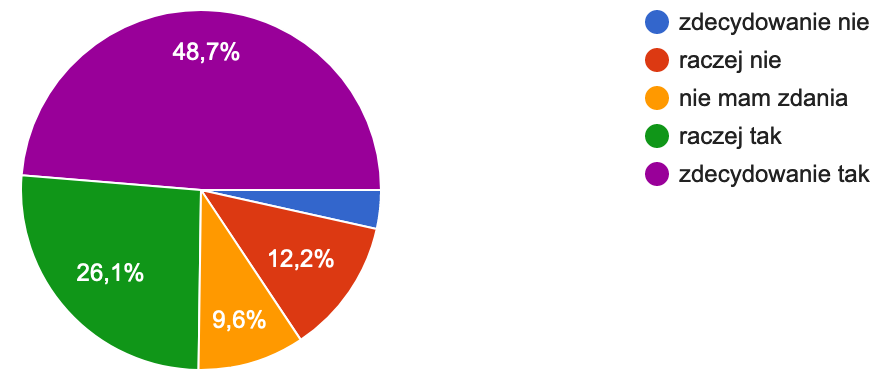
\includegraphics[width=9cm]{wyniki/19_popiera_dzialania}
    \caption{ 19 popiera dzialania }
\end{figure}

%  20 odczuwa satys
\begin{figure}
    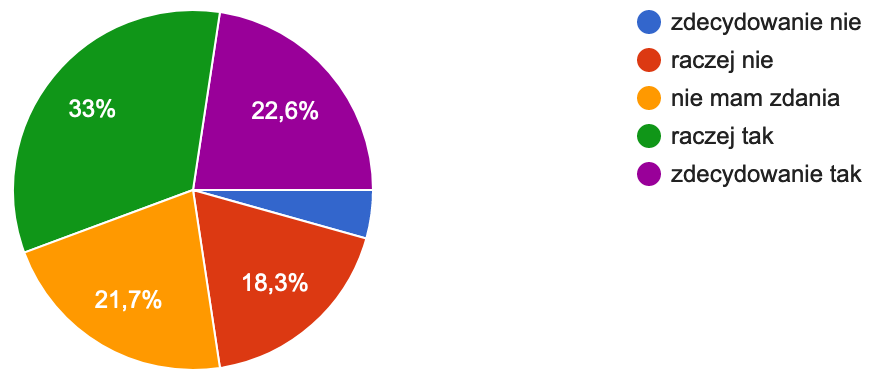
\includegraphics[width=9cm]{wyniki/20_odczuwa_satys}
    \caption{ 20 odczuwa satys }
\end{figure}